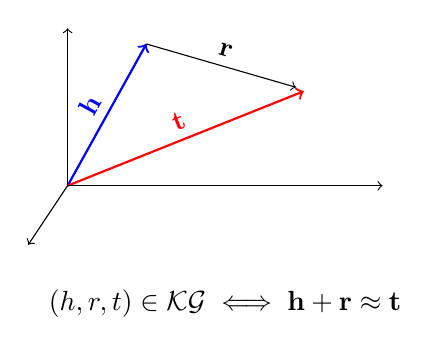
\begin{tikzpicture}
[   cnode/.style={draw=black,fill=#1,minimum width=3mm,circle},
    rnode/.style={draw=black,fill=#1,minimum width=6mm, minimum height=5mm, rectangle}
]
    
    \draw[->,blue,thick] (0,0) -- node[above, sloped]{$\mathbf{h}$} (1, 1.8);
    \draw[->,red, thick] (0,0) -- node[above, sloped]{$\mathbf{t}$} (3, 1.2);
    \draw[->] (1,1.8) -- node[above, sloped]{$\mathbf{r}$} (2.9, 1.25);
    
    \draw[->] (0,0) -- (4,0);
    \draw[->] (0,0) -- (-0.5, -0.75);
    \draw[->] (0,0) -- (0,2);
    
    \node at (2, -1.5) {$(h, r, t) \in \mathcal{KG} \iff \mathbf{h} + \mathbf{r} \approx \mathbf{t} $};
\end{tikzpicture}